\documentclass[12pt,a4paper]{article}
\raggedbottom

\usepackage{ugmath}
\usepackage{float}
\usepackage{placeins}
\usepackage[labelfont=bf,labelsep=space]{caption}
\usepackage{pdfpages}
\usepackage{tikz-cd}
\usepackage{amsthm}
\renewcommand{\Tr}{\operatorname{Tr}}
\newcommand{\llaves}[1]{\{#1\}}
\newcommand{\parentesis}[1]{\left(#1\right)}
\newcommand{\corchetes}[1]{\left[#1\right]}
\newcommand{\llavesgrande}[1]{\big\{#1\big\}}
\newcommand{\llavesgrandes}[1]{\left\{#1\right\}}


\begin{document}

    \thispagestyle{empty}
    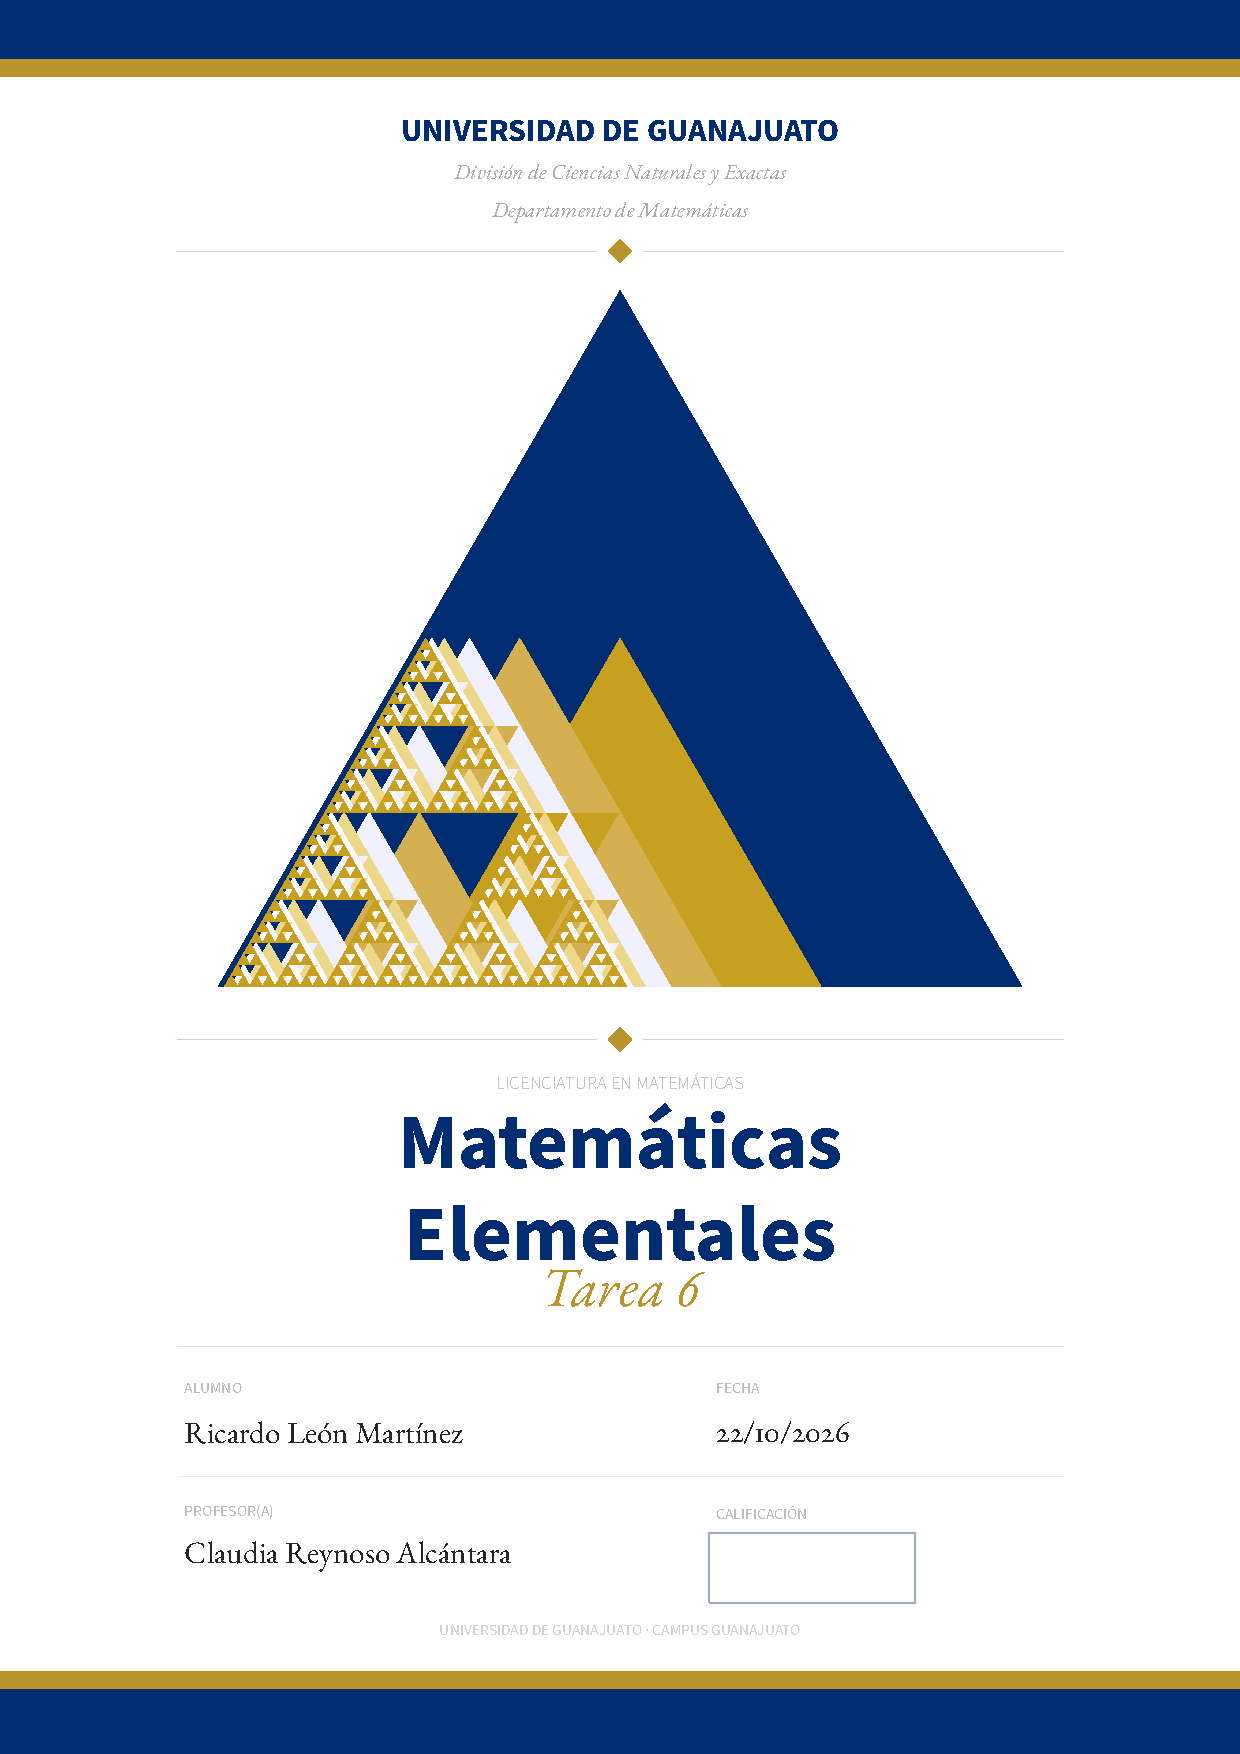
\includepdf[pages=1]{portada.pdf}

    \begin{problema}
        Sean $a,b,c\in\Z$ tales que $a>b$ y $c>0$. Demuestra que $ac>bc$.
    \end{problema}

    \begin{proof}
        Como $b<a$, sumando $-b$ a ambos lados de la desigualdad se obtiene $0=b+(-b)<a+(-b)=a-b$. Como $a-b>0$ y
        $c>0$, por la cerradura de los enteros positivos bajo el producto, $(a-b)c>0$. Por la distributividad y la
        regla de signos,
        \begin{equation*}
            (a-b)c=ac+(-b)c=ac+\big(-(bc)\big),
        \end{equation*}
        así que $0<ac+\big(-(bc)\big)$. Sumando $bc$ a ambos lados y usando la asociatividad de la suma,
        \begin{equation*}
            bc=0+bc<\Big(ac+\big(-(bc)\big)\Big)+bc=ac+\Big(\big(-(bc)\big)+bc\Big)=ac+0=ac.
        \end{equation*}
        Por lo tanto $ac>bc$.
    \end{proof}

    \begin{problema}
        Sean $a,b,c\in\Z$ tales que $a>b$ y $c<0$. Demuestra que $ac<bc$.
    \end{problema}

    \begin{proof}
        Como $b<a$, sumando $-b$ a ambos lados se obtiene $0<a-b$. Como $c<0$, sumando $-c$ a ambos lados se obtiene
        $0=c+(-c)<0+(-c)=-c$. Por la cerradura de los enteros positivos bajo el producto, $(a-b)(-c)>0$.

        Para todo $x\in\Z$ se tiene $-(-x)=x$, pues $(-x)+x=0$ y el inverso aditivo de $-x$ es único. Por la
        distributividad y la regla de signos,
        \begin{equation*}
            (a-b)(-c)=a(-c)+(-b)(-c)=-(ac)+\Big(-\big(b(-c)\big)\Big)=-(ac)+\Big(-\big(-(bc)\big)\Big)=-(ac)+bc.
        \end{equation*}
        Así que $0<bc+\big(-(ac)\big)$. Sumando $ac$ a ambos lados y usando la asociatividad de la suma,
        \begin{equation*}
            ac=0+ac<\Big(bc+\big(-(ac)\big)\Big)+ac=bc+0=bc.
        \end{equation*}
        Por lo tanto $ac<bc$.
    \end{proof}

    \textbf{Definición 1.} Sea $a\in\Z$. Definimos el \textbf{valor absoluto} de $a$ como
    \begin{equation*}
        |a|:=\begin{cases}
            a & \text{si } a\ge0,\\
            -a & \text{si } a<0.
        \end{cases}
    \end{equation*}

    \begin{problema}
        Demuestra que si $a,b\in\Z$, entonces $|ab|=|a||b|$.
    \end{problema}

    \begin{proof}
        Todo entero es cero, positivo o negativo, y para $x\in\Z$ se tiene
        \begin{equation}\label{eq:signo-opuesto}
            x>0 \iff -x<0, \qquad\qquad x<0 \iff -x>0,
        \end{equation}
        lo cual se obtiene sumando $-x$ o $x$ a ambos lados de la desigualdad correspondiente y usando que
        $-(-x)=x$, pues $(-x)+x=0$ y el inverso aditivo es único. Además $x\cdot0=0$ para todo $x\in\Z$, pues si $x=[(p,q)]$, entonces $x\cdot[(1,1)]=[(p+q,q+p)]=0$.

        Procederemos por casos.

        Si $a=0$ o $b=0$, entonces $ab=0$, por la conmutatividad del producto. Como $0\ge0$, se tiene $|0|=0$, así
        que $|ab|=0$. Además, uno de $|a|$, $|b|$ es $0$, así que $|a||b|=0=|ab|$.

        Si $a>0$ y $b>0$, por la cerradura de los enteros positivos bajo el producto $ab>0$. Entonces $|ab|=ab=|a||b|$.

        Si $a>0$ y $b<0$, por \eqref{eq:signo-opuesto} $-b>0$, así que $a(-b)>0$ por la cerradura de los enteros
        positivos. Por la regla de signos $a(-b)=-(ab)$, así que $-(ab)>0$, y por \eqref{eq:signo-opuesto} $ab<0$.
        Por lo tanto
        \begin{equation*}
            |ab|=-(ab)=a(-b)=|a||b|.
        \end{equation*}

        Si $a<0$ y $b>0$, el caso anterior aplicado a $b$ y $a$, junto con la conmutatividad del producto, da
        $|ab|=|ba|=|b||a|=|a||b|$.

        Si $a<0$ y $b<0$, por \eqref{eq:signo-opuesto} $-a>0$ y $-b>0$, así que $(-a)(-b)>0$. Por la regla de signos,
        \begin{equation*}
            (-a)(-b)=-\big(a(-b)\big)=-\big(-(ab)\big)=ab,
        \end{equation*}
        así que $ab>0$ y
        \begin{equation*}
            |ab|=ab=(-a)(-b)=|a||b|.
        \end{equation*}

        En todos los casos $|ab|=|a||b|$.
    \end{proof}

    \begin{problema}
        Sean $a,b\in\Z$. Demuestra que $|a+b|\le|a|+|b|$.
    \end{problema}

    \begin{proof}
        Si $x,y\in\Z$ cumplen $x\ge0$ y $y\ge0$, entonces $x+y\ge0$. En efecto, si
        $x=0$ o $y=0$, la suma es igual al otro sumando, y si $x,y>0$, la suma es positiva por la cerradura de los
        enteros positivos bajo la suma. Además, si $y-x\ge0$, entonces $x\le y$, pues si $y-x=0$ se tiene $y=x$, y si
        $y-x>0$, sumando $x$ a ambos lados se obtiene $x<(y-x)+x=y$.

        Para todo $x\in\Z$ se cumple
        \begin{equation}\label{eq:abs-mas-menos}
            |x|-x\ge0 \qquad\text{y}\qquad |x|+x\ge0.
        \end{equation}
        En efecto, si $x\ge0$, entonces $|x|-x=x-x=0$ y $|x|+x=x+x\ge0$. Si $x<0$, entonces $|x|=-x>0$, así que
        $|x|+x=(-x)+x=0$ y $|x|-x=(-x)+(-x)>0$ por la cerradura de los enteros positivos bajo la suma.

        Si $a+b\ge0$, entonces $|a+b|=a+b$ y, por la asociatividad y conmutatividad de la suma,
        \begin{equation*}
            \big(|a|+|b|\big)-|a+b|=\big(|a|-a\big)+\big(|b|-b\big),
        \end{equation*}
        que es $\ge0$ por \eqref{eq:abs-mas-menos}. Si $a+b<0$, entonces $|a+b|=-(a+b)$ y, como $-\big(-(a+b)\big)=a+b$,
        \begin{equation*}
            \big(|a|+|b|\big)-|a+b|=\big(|a|+|b|\big)+(a+b)=\big(|a|+a\big)+\big(|b|+b\big),
        \end{equation*}
        que también es $\ge0$ por \eqref{eq:abs-mas-menos}. En ambos casos $\big(|a|+|b|\big)-|a+b|\ge0$, es decir,
        $|a+b|\le|a|+|b|$.
    \end{proof}

    \textbf{Definición 2.} Sean $a,b\in\Z$, $a\neq0$. Un \textbf{máximo común divisor} de $a$ y $b$ es un número
    natural $n\in\N$ que satisface lo siguiente:
    \begin{enumerate}[label=\alph*)]
        \item $n$ divide a $a$ y $n$ divide a $b$, y
        \item si $m\in\N$ divide a $a$ y divide a $b$, entonces $m$ divide a $n$.
    \end{enumerate}

    \begin{problema}
        Demuestra que si $p\in\N$ es primo, entonces para todo $a\in\Z-\{0\}$ se satisface alguna de las siguientes
        condiciones: $\operatorname{mcd}(p,a)=1$ o $\operatorname{mcd}(p,a)=p$.
    \end{problema}

    \begin{proof}
        Sea $a\in\Z-\{0\}$. Como $p\neq0$, el máximo común divisor de $p$ y $a$ existe y es único. Sea
        $n=\operatorname{mcd}(p,a)\in\N$. Como $n$ divide a $p$, existe $k\in\Z$ tal que $p=nk=kn$. Si $k=0$, entonces $p=0$, y si $k<0$,
        por el Ejercicio~1 aplicado a $0>k$ y $n>0$ se tiene $p=kn<0\cdot n=0$. Ambos casos contradicen $p>0$, así
        que $k>0$, es decir, $k\in\N$. Así que $p=nk$ con $n,k\in\N$, es
        decir, $n$ es un divisor de $p$ en $\N$. Como $p$ es primo, sus únicos divisores son $1$ y $p$, por lo
        tanto $n=1$ o $n=p$.
    \end{proof}

    \begin{problema}
        Sea $p\in\Z$ con $p>0$ y sean $a=p^3+2p^2+2p+2$, $d=p+1$. Encuentra $q,r\in\Z$ tales que $a=qd+r$ y
        $0\le r<|d|$.
    \end{problema}

    \begin{proof}[Solución]
        Sean $q=p^2+p+1$ y $r=1$. Por la distributividad, la asociatividad y la conmutatividad de la suma y el
        producto en $\Z$,
        \begin{equation*}
            qd+r=(p^2+p+1)(p+1)+1=(p^3+p^2+p)+(p^2+p+1)+1=p^3+2p^2+2p+2=a.
        \end{equation*}
        Como $p>0$ y $1>0$, por la cerradura de los enteros positivos bajo la suma $d=p+1>0$, así que $|d|=d$. Además
        $0<1$, y como $(p+1)-1=p>0$, sumando $1$ a ambos lados se obtiene $1<p+1=|d|$. Por lo tanto
        \begin{equation*}
            q=p^2+p+1, \qquad r=1
        \end{equation*}
        satisfacen $a=qd+r$ y $0\le r<|d|$.
    \end{proof}

    \begin{problema}
        Sean $a,b$ enteros positivos tales que $b$ no divide a $a$. Sea $b=r_0$. Sabemos, por el algoritmo de la
        división, que existen únicos $q_0,r_1$ tales que $a=r_0q_0+r_1$ y $0<r_1<r_0$. Para $j\ge1$, sean
        $q_j,r_{j+1}$ tales que
        \begin{equation*}
            r_{j-1}=r_jq_j+r_{j+1}, \qquad 0<r_{j+1}<r_j.
        \end{equation*}
        Demuestra que existe $n\in\N$ tal que $r_{n+1}=0$ y $r_n\neq0$. Demuestra que $r_n$ es el máximo común
        divisor de $a$ y $b$.
    \end{problema}

    \begin{proof}
        El algoritmo de la división aplicado a $r_{j-1}$ y $r_j$ requiere $r_j\neq0$ y garantiza
        $0\le r_{j+1}<r_j$, así que $r_{j+1}$ está definido mientras $r_j\neq0$. Además $r_0=b>0$, y $r_1>0$ porque
        $b$ no divide a $a$.

        Procederemos por contradicción para probar que algún $r_j$ es cero. Supongamos que $r_j\neq0$ para todo
        $j\ge0$. Entonces todos los $r_j$ están definidos y son positivos, y el conjunto
        $S=\{r_j : j\ge0\}\subseteq\Z_{>0}$ es no vacío y está acotado inferiormente por $0$. Por el principio del
        buen orden, $S$ tiene un elemento mínimo $r_k$. Pero $r_{k+1}\in S$ y $r_{k+1}<r_k$, lo cual contradice la
        minimalidad de $r_k$. Por lo tanto el conjunto $\{j\in\N : r_j=0\}$ es no vacío, y por el principio del buen
        orden en $\N$ tiene un elemento mínimo $m$. Como $r_1\neq0$, se tiene $m\neq1$, así que $m=n+1$ para algún
        $n\in\N$. Por la minimalidad de $m$, $r_n\neq0$, y $r_{n+1}=0$.

        Si $e\in\Z-\{0\}$ divide a $x$ y a $y$, entonces $e$ divide a $ux+vy$ para cualesquiera $u,v\in\Z$, pues si
        $x=ex'$ y $y=ey'$, por la distributividad, la asociatividad y la conmutatividad del producto,
        \begin{equation}\label{eq:combinacion}
            ux+vy=u(ex')+v(ey')=e(ux'+vy').
        \end{equation}

        Como $r_n>0$, identificamos $r_n$ con un número natural. Procederemos por inducción sobre $k$ para probar que
        para todo $k\in\N$ con $k\le n$, $r_n$ divide a $r_{n-k+1}$ y a $r_{n-k}$. Si $k=1$, se tiene $r_n=r_n\cdot1$ y
        $r_{n-1}=r_nq_n+r_{n+1}=r_nq_n$, así que $r_n$ divide a $r_n$ y a $r_{n-1}$. Supongamos que $k<n$ y que $r_n$
        divide a $r_{n-k+1}$ y a $r_{n-k}$. Como $n-k\ge1$,
        \begin{equation*}
            r_{n-k-1}=r_{n-k}\,q_{n-k}+r_{n-k+1},
        \end{equation*}
        y por \eqref{eq:combinacion} $r_n$ divide a $r_{n-k-1}$. Así que $r_n$ divide a $r_{n-(k+1)+1}=r_{n-k}$ y a
        $r_{n-(k+1)}$. Por inducción, tomando $k=n$, $r_n$ divide a $r_1$ y a $r_0=b$. Como $a=r_0q_0+r_1$, por
        \eqref{eq:combinacion} $r_n$ divide a $a$.

        Sea $m\in\N$ tal que $m$ divide a $a$ y a $b$. Procederemos por inducción sobre $j$ para probar que para todo
        $j\in\N$ con $j\le n$, $m$ divide a $r_{j-1}$ y a $r_j$. Si $j=1$, $m$ divide a $r_0=b$ y, como
        $r_1=a+(-q_0)r_0$, por \eqref{eq:combinacion} $m$ divide a $r_1$. Supongamos que $j<n$ y que $m$ divide a
        $r_{j-1}$ y a $r_j$. Como $r_{j+1}=r_{j-1}+(-q_j)r_j$, por \eqref{eq:combinacion} $m$ divide a $r_{j+1}$. Así
        que $m$ divide a $r_j$ y a $r_{j+1}$. Por inducción, tomando $j=n$, $m$ divide a $r_n$.

        Por lo tanto $r_n$ satisface las condiciones a) y b) de la Definición 2, y por la unicidad del máximo común
        divisor, $r_n=\operatorname{mcd}(a,b)$.
    \end{proof}

\end{document}
